%!TEX root = ../thesis.tex
\chapter{Introduction}  % Main chapter title
\label{cha:introduction}

%----------------------------------------------------------------------------------------
%    SECTION 1
%----------------------------------------------------------------------------------------

\section{Main Section 1}


MR relation ship image arXiv:1506.05097~\citet{chen_probabilistic_2016}

\begin{figure}
    \centering
    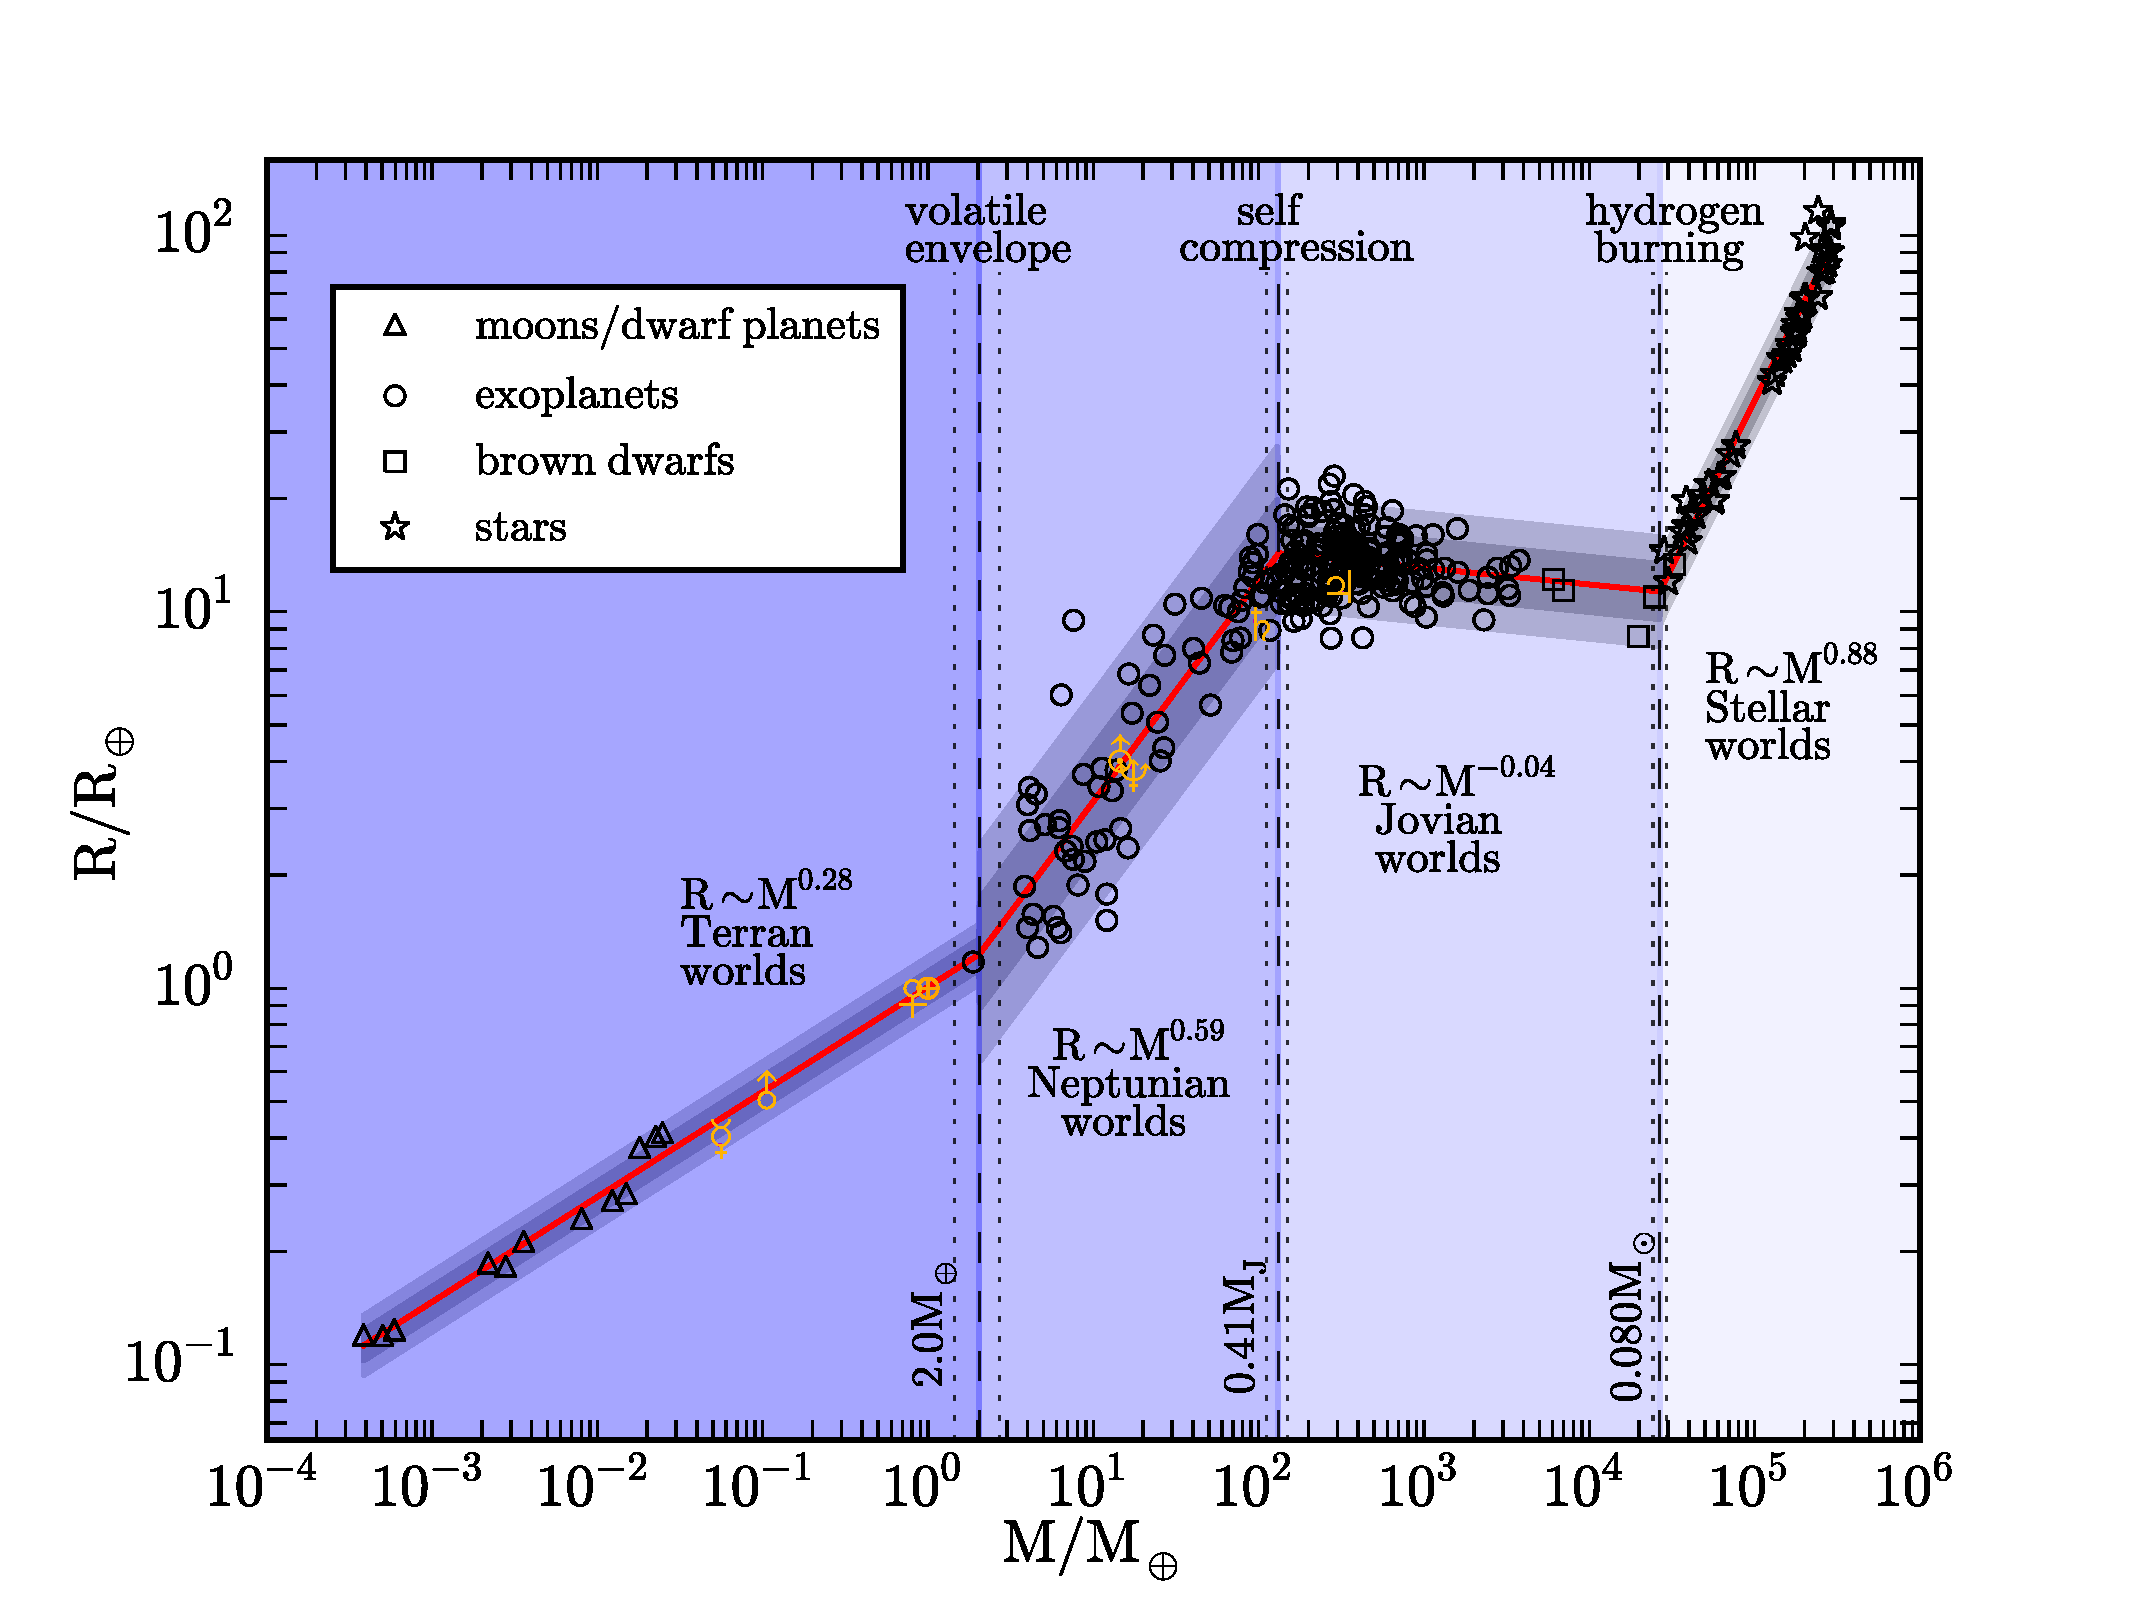
\includegraphics[width=0.7\linewidth]{./figures/introduction/plt_overlay_add.pdf}
    \caption{M-R relationship~\citet{chen_probabilistic_2016}}
    \label{fig:pltoverlayadd}
\end{figure}

Santos et al 2017 \todo{read and quote}

%-----------------------------------
%    SUBSECTION 1
%-----------------------------------
\subsection{Subsection 1}


%-----------------------------------
%    SUBSECTION 2
%-----------------------------------

\subsection{Subsection 2}

%----------------------------------------------------------------------------------------
%    SECTION 2
%----------------------------------------------------------------------------------------

\section{Main Section 2}


Spectral Disentangling techniques
- PSOAP
- Differencing Fruluga
- Templates?


2D-cross-correlation?   piskorz 2016


\section{Recent detections in Companion spectra.}


Birkby


\subsection{model fitting transit stars (not actual title, more other similar methods)}
There are other situations in which to determine the presence of faint secondary spectra, such as, identifying the presence of any background or companion stars of transiting planet candidates. Many astronomical phenomena such as grazing eclipsing, a giant primary star eclipsed by a dwarf or a background star can produce signals indistinguishable from planetary transits. Efforts to characterize the false positive probability (FPP) among Kepler planet candidates is as high as $\sim35\%$~\citep{santerne_sophie_2012}. The presence of unknown companions or background stars decreases the dimming effect from the planet transit leading to smaller planetary radius. Where multiple stars are present there may also be ambiguity on which star hosts the planet.~\citet{kolbl_detection_2015} developed a method for detecting the presences of faint secondary lines in optical stellar spectra by matching observations to the SpecMatch library of stellar spectra. Identifying the spectroscopic evidence of a secondary star for 63/1\,160 California \emph{Kepler} Survey objects of Interest (KOI).


For transiting planets that presence of a background star or a companion star causes problems in characterizing the planet. Being able to detect spectra signal of the a faint second spectra in double-lined spectroscopic binaries.
For example eclipsing binaries,
A dim binary system companion or a giant planet around a background star can mimic the transit of a small Earth-like planet on a foreground star.






\subsection{Earths atmosphere}
While the Earth's atmosphere is important for an Astronomer's lungs, it can be a nuance for their ground-based observations. As light form astronomical sources passes through the atmosphere, its molecular components absorb some of the light, changing spectral components observed  by imprinting a transmission spectrum of our atmosphere. The \ce{H2O} absorption is a key example as it defines the photometric and spectroscopic bands in the \nir{}. \missingfigure{example to point to}.

The correction of observations from the contamination of Earth's atmosphere is a complex process. The transmission is variable on many different time scales, the water vapour change is rapid, concentrations of atmospheric constituents, to seasonal and longer. Such as the increase in atmospheric \ce{CO2} causing anthropamorphic climate change this requires 6\% change to \ce{CO2} line depths since 2000 Molecfit paper? There is also variation with airmass, which depends on the observation angle in the sky and changes as targets move across the sky during the night.

other constituents, \ce{CO}, \ce{CO2}, \ce{CH4} \ldots{}, angle of observations.

An important consideration in the detecting the constituents of planetary atmospheres is the characterization and removal of Earths telluric lines.

e.g.\ 50\% error in \ce{CO2} detection on Mars atmosphere


Recently \citet{ulmer-moll_telluric_2018} compared the telluric correction possible from three different synthetic telluric software against the standard star model. Molecfit, a software from ESO was the most.

This is a growing field and there are other software available too\ldots{}


Water vapour content has rapid variability. Works such as Snellen 2011, \ldots{} \ldots{}  model the telluric variation during a observations to remove telluric lines and detect planetary lines.

\todo{finish this}


Telluric absorption map
\begin{figure}
    \centering
    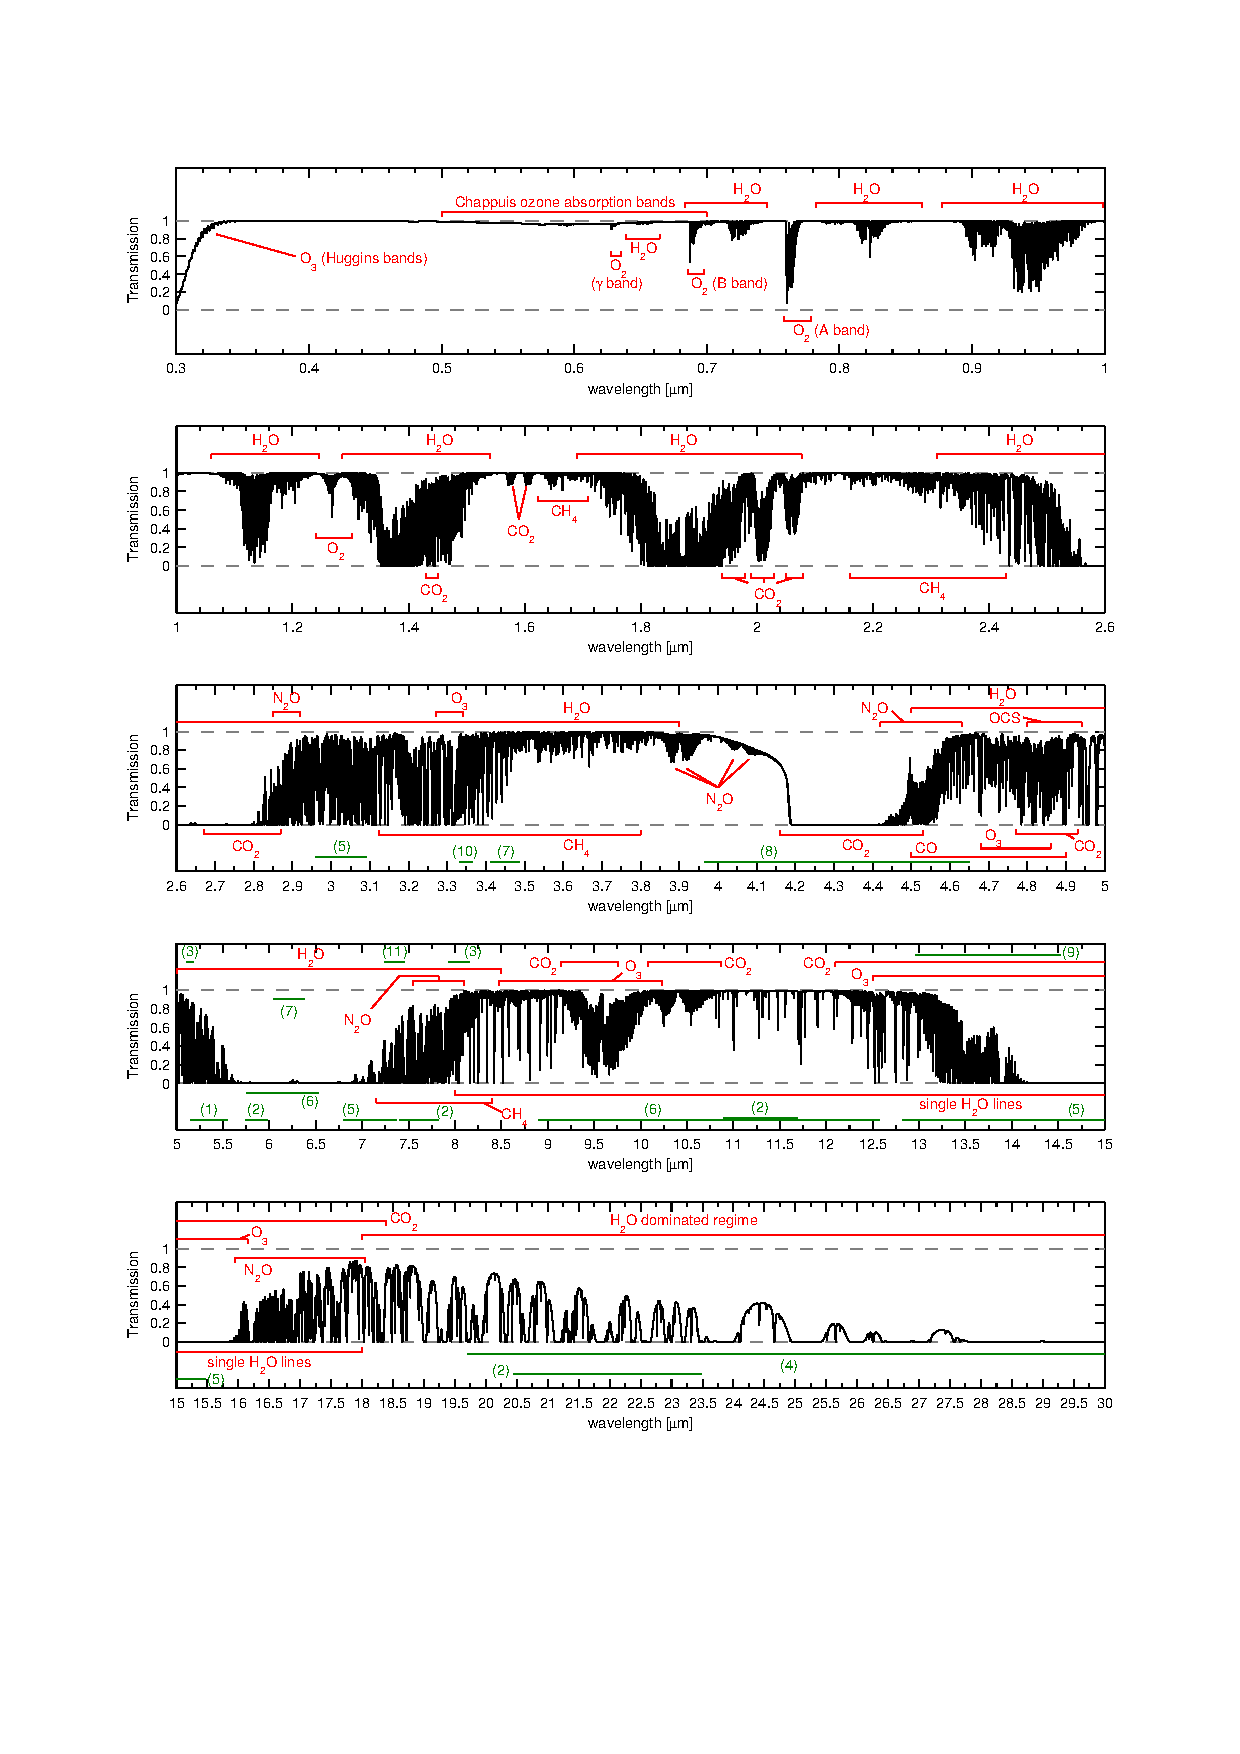
\includegraphics[width=0.9\linewidth]{figures/advanced_material/cropped_molecfit_absorbtion}
    \caption{Reproduction of Figure~1 of \citet{smette_molecfit_2015} showing telluric absorption form 0.30 \um. Original caption:}
    \label{fig:croppedmolecfitabsorbtion}
\end{figure}
\todo{Add original caption to \ref{fig:croppedmolecfitabsorbtion}}




\section{Paper Introduction}
\label{sec:intro}
Brown dwarfs (BDs) are sub-stellar objects unable to achieve hydrogen fusion, with masses around \(13-80~\textrm{M}_{jup} \)~\citep{chabrier_theory_2000}, bridging the gap between low-mass stars and giant planets. Without sustained fusion, brown-dwarfs cool down over time with an age-dependent cooling rate. Therefore, there is an inherent degeneracy between the mass, age and luminosity of a given BD\citep{burrows_nongray_1997}. This degeneracy may be broken by observation of several parameters, for instance when a BD is in a binary system with a main sequence host star, using both the host stars age and the masses derived from the dynamical motion.

A paucity of BD companions exists in short period orbits around Sun-like stars (\(\lesssim5 \)\,AU), compared to stellar or planetary companions, termed the \emph{brown dwarf desert}~\citep{halbwachs_exploring_2000,zucker_analysis_2001,sahlmann_search_2011}. As the number of known BDs orbiting solar type stars is low, the characterization of benchmark BDs in the brown dwarf desert~\citep[e.g.][]{crepp_trends_2016} is beneficial in understanding this sub-stellar population and to help constrain formation and evolution theories~\citep{whitworth_formation_2007}. The BD desert also provides a greater challenge as it reduces the amount of good BD candidates to study.

BDs in binary systems, unlike free-floating BDs, allow for the determination of their masses, when complemented with radial velocity ({RV}) and astrometry measurements. The {RV} technique provides the mass lower-limit (\mtwosini{}) of binary and planetary companions, while complementary astrometry measurements can often provide mass upper-limits~\citep[e.g.][]{sahlmann_search_2011}. Measuring or tightening the constraints of BD masses improves the understanding of mass dependence on BD formation processes. For instance, there is growing evidence that the larger giant planets and BD companions do not follow the well known metallicity-giant planet correlation seen in main-sequence stars with planets~\citep[e.g.][]{santos_spectroscopic_2004,santos_observational_2017, maldonado_searching_2017}. Photometry along with stellar evolution models~\citep[e.g.][]{baraffe_evolutionary_2003,allard_btsettl_2013} can also be used to estimate the mass of BD companions~\citep[e.g.][]{moutou_eccentricity_2017} if there is sufficient orbital separation, and a precise determination of the age~\citep{soderblom_ages_2010}.

Recently, there has been a renewed interest in BD candidates triggered by exoplanetary searches. While several works found similar properties on the two populations, like a similar density~\citep{hatzes_definition_2015}, others found intriguing differences. One of the most recent is the different host metallicity of the Brown Dwarf and giant planet populations~\citep{santos_observational_2017, schlaufman_evidence_2018}, a very strong hint of different formation mechanisms.

Spectral observations of binary systems contain the spectra of both bodies, in proportion to their flux ratio, and Doppler shifted relative to each other due to their orbital motion. One technique to recover the spectra of the companion is secondary reconstruction through a differential spectrum~\citep{ferluga_separating_1997}. Spectra from different phases are shifted to the host stars rest frame and subtracted to mutually cancel out the spectrum of the host star allowing the faint companion spectra to become visible. Advances in high-resolution and near-infrared (\nir{}) capabilities should enable this technique to be applied to BDs and planet companions, in which smaller {RV} shifts can be resolved and the contrast ratio of the smaller companion is improved.

Observing in the \nir{}is specifically desirable for the cooler sub-stellar and giant planet companions as their thermal emission is stronger in the infrared compared to the optical. This improves the contrast ratio between the host star and companion, providing favourable conditions for their detection and spectral separation. CRIRES, a high resolution \nir{}spectrograph, has made many prominent advances in recent years with the detection of atmospheric constituents, such as \(\textrm{CO} \) and \(\textrm{H}_{2}\textrm{O} \), atmospheric winds and thermal profiles, rotation and orbital motion, for both transiting and non-transiting planets~\citep[e.g.][]{snellen_orbital_2010, brogi_signature_2012, rodler_weighing_2012, dekok_detection_2013, brogi_carbon_2014, snellen_fast_2014, piskorz_evidence_2016, brogi_rotation_2016, birkby_discovery_2017}.

The higher temperature and relatively larger size of BDs compared to giant-planets makes the development of spectral recovery techniques for BD companions a logical step towards the spectroscopic detection of planetary atmospheres. There has been the recent installation and continued development of many new high-resolution \nir{}spectrographs, such as, {CARMENES}~\citep{quirrenbach_carmenes_2014}, NIRPS~\citep{bouchy_nearinfrared_2017} or SPIRou~\citep{artigau_spirou_2014}, as well as, the CRIRES+~\citep{dorn_crires_2016} upgrade. These new instruments motivate the study of \nir{}-oriented methodologies for spectral recovery, and are of high importance due to the larger planet-to-star flux ratio provided by near-IR compared to the visible.

{\rd{} The search and detection of faint secondary spectra is not only relevant to planetary atmospheres.~\citet{kolbl_detection_2015} developed a method to detect the presence of optical secondary spectra down to a flux ratio of 1\% in the hosts of \emph{Kepler} transit candidates. The presence of which can cause ambiguities in the system configuration, and increase the uncertainty of the measured planet radius. The characterization of the false positive probability rate for Kepler has been found to be as high as  \(\sim\)35\%~\citet{santerne_sophie_2012}.}

In this paper we apply two different techniques on FGK stars with BD companions with the aim to spectroscopically detect their companions. In Sect.~ref{sec:data} we present the observations and reduction process as well as the spectral models used in this work. In Sect.~ref{sec:specdiff} we explain the differential spectral technique and its applicability to these observations while in Sect.~ref{sec:results} we apply companion recovery using a \textchisquared approach. In Sect.~ref{sec:discussion} we discuss our results and in Sect.~ref{sec:conclusions} we present our conclusions.
